\documentclass[serif,mathserif]{beamer}
\usepackage[portuguese]{babel}
\usepackage[utf8]{inputenc}
\usepackage{amsmath, amsfonts, epsfig, xspace}
\usepackage{algorithm,algorithmic}
\usepackage{pstricks,pst-node}
\usepackage{multimedia}
\usepackage[normal,tight,center]{subfigure}
\setlength{\subfigcapskip}{-.5em}
\usepackage{beamerthemesplit}
\usetheme{lankton-keynote}
\setbeamerfont{title}{size=\large}

\newcommand{\CcImageBy}[1]{%
  
\includegraphics[scale=#1]{src/img/creative_commons/cc_by_30.pdf}%
}
\newcommand{\CcImageSa}[1]{%
  
\includegraphics[scale=#1]{src/img/creative_commons/cc_sa_30.pdf}%
}
\newcommand{\CcGroupBySa}[2]{% zoom, gap
  \CcImageBy{#1}\hspace*{#2}\CcImageSa{#1}%
}
\newcommand{\CcLongnameBySa}{Attribution-ShareAlike}
\newcommand{\CcNote}[1]{% longname
  This work is licensed under the \textit{Creative Commons #1 3.0 License}.%
}

\author[Alessandro Palmeira\\ \and Itai Soares]{Alessandro Palmeira\\ \and Itai Soares}

\title[Instituto de Matemática e Estatística - USP\hspace{2em}\insertframenumber/\inserttotalframenumber]{Acompanhamento musical em tempo real utilizando múltiplas performances como referência}

\date{22 de Setembro de 2016} %leave out for today's date to be insterted

\institute{MAC6917 Topics in Sound and Music Computing: Music Information Retrieval}


\begin{document}


\begin{frame}
  \titlepage
  \begin{center}
    \CcGroupBySa{0.83}{0.95ex}\\
    {\tiny\CcNote{\CcLongnameBySa}}
  \end{center}
\end{frame}

\section{Apresentação}
\begin{frame}
  \frametitle{Apresentação}
  Este seminário será uma apresentação do artigo \emph{Real-time music tracking using multiple performances as a reference} de Andreas Arzt e Gerhard Widmer que ganhou o \emph{Best Paper Award} na  \emph{International Society for Music Information Retrieval Conference} de 2015.
\end{frame}

\section{Introdução}  % add these to see outline in slides

\begin{frame}
  \frametitle{Algoritmos de Acompanhamento em Tempo Real}
  Existem desde a década de 1980 e ainda atraem bastante pesquisa.\pause\\
  Essa tecnologia tem sido usado em aplicações práticas.\pause
  %Colocar vídeo do SmartMusic(1985) aqui
  \begin{itemize}
    \item Antescofo\\\pause
    \item Tonara
  \end{itemize}
\end{frame}

\begin{frame}
  \frametitle{Estratégias utilizadas}
  \begin{itemize}
    \item Inicia-se com uma representação simbólica, como um arquivo MIDI ou MusicXML\\\pause
    \item Converte-o para um arquivo de áudio, usando um softare sintetizador\pause
      \begin{itemize}
        \item Sabe-se o tempo de cada evento\\\pause
        \item O problema se reduz a um alinhamento áudio-áudio
      \end{itemize}
  \end{itemize}
\end{frame}

\begin{frame}
  \frametitle{Nova estratégia}
  \begin{itemize}
    \item Primeiramente utilizamos uma outra performance da música e a alinhamos com a partitura automaticamente\\\pause
    \item Depois, utilizamos essa ``performance anotada'' como nova representação para o processo de rastreamento online\pause
  \end{itemize}

  %inserir figura src/img/2-Figure1-1.png

%\vspace{5mm} %5mm vertical space

  As motivações são:\pause
  \begin{itemize}
    \item Qualidade das \emph{features} extraídas\\\pause % O arquivo de áudio tem qualidade maior do que uma síntese
    \item Complexidade perdida na notação musical, que aparece em uma performance\pause % Como trilos, por exemplo
  \end{itemize}
  Porém, temos também uma desvantagem:\pause
  \begin{itemize}
    \item A qualidade do processo fica dependente da performance\\
  \end{itemize}
\end{frame}


\section{Descrição dos dados}
\begin{frame}
  \frametitle{Visão Geral}
  \begin{center}
    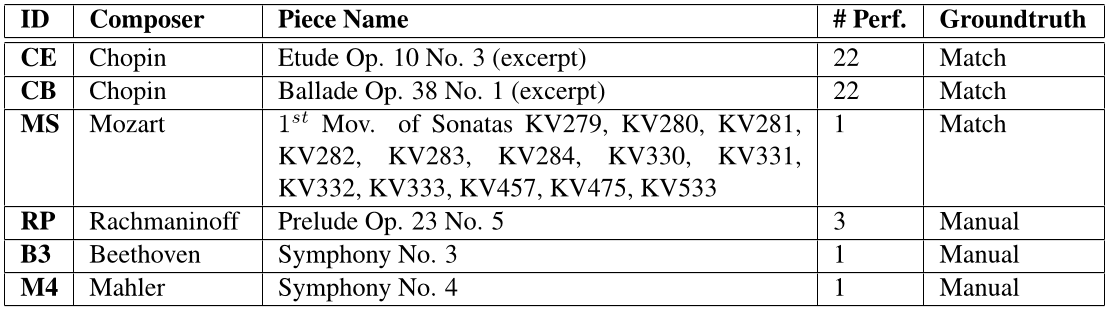
\includegraphics[width=\textwidth]{src/img/1-Table1-1.png}
  \end{center}
\end{frame}

\section{Acompanhamento padrão}
\begin{frame}
  \frametitle{Acompanhamento padrão baseado em representação simbólica musical}
  Abordagem baseada no algoritmo \emph{Dynamic Time Warping (DTW)} com algumas extensões:\pause % que possibilitam a aplicação em rastreamento online. [artigo 10]
  \begin{itemize}
    \item O caminho é computado de maneira incremental\\\pause
    \item A complexidade é reduzida para ser linear no tamanho da entrada\pause
    \item Utiliza a estratégia \emph{backward-forward} %reconsidera decisoes passadas, aumenta robustez [artigo 4]
    \item Modelo simples de andamento (\emph{Simple tempo model}) % aumenta a habilidade de o algoritmo lidar com diferencas no Andamento [artigo 3]
  \end{itemize}
\end{frame}



\begin{frame}
  \frametitle{Dúvidas?}
  \begin{itemize}
    \item Os slides estão disponíveis em \url{https://github.com/compmusMIR}
  \end{itemize}
\end{frame}

\begin{frame}
  \frametitle{Referências}
  \small
  Apresentação:\\
  \vspace{2mm}
  \url{https://www.semanticscholar.org/paper/Real-Time-Music-Tracking-Using-Multiple-Arzt-Widmer/0223b9d27de14f2c158028290782a937ff537786}


\end{frame}

\end{document}